\subsection{Pigeon}
Pigeons occur worldwide except in the coldest regions and the most remote islands. About 250 species are known; two-thirds of them occur in tropical Southeast Asia, Australia, and the islands of the western Pacific, but the family also has many members in Africa and South America and a few in temperate Eurasia and North America. All members of the family suck liquids, rather than sip and swallow as do other birds, and all pigeon parents feed their young “pigeon’s milk,” the sloughed-off lining of the crop, the production of which is stimulated by the hormone prolactin. The nestling obtains this “milk” by poking its bill down the parent’s throat.
\begin{figure}[htp]
    \centering
    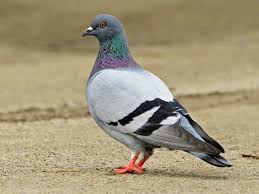
\includegraphics{images (12).jpeg}
    \caption{Rock Pigeon}
\end{figure}